\chapter[Summary, conclusions, and perspectives]{\texorpdfstring{Summary, conclusions, and\\ perspectives}{Summary, conclusions, and perspectives} }\label{ch:conclusions}

This Thesis presented the measurement of the \pt-differential \ds/\dpl production-yield ratio in proton-proton collisions at \thirteen, performed with the upgraded ALICE detector and the data collected during the LHC Run~3 data-taking period. This allowed the study of the charm-quark hadronisation (i.e., the transition from a colour-charged quark into colour neutral hadrons) via strange over non-strange charm meson production-yield ratios.

The analysis was performed via the full reconstruction of displaced decay topologies through the same hadronic decay channel $\ds, \dpl \rightarrow \phi\pi^+\rightarrow\mathrm{K^+K^-\pi^+}$. Multiclass Machine Learning models using the Boosted Decision Tree algorithm provided by the XGBoost library were employed to enhance the selection efficiency of the signal candidates and to reduce the combinatorial background. Additionally, they were used to increase the relative contribution of prompt \ds and \dpl mesons (i.e., those directly produced in the hadronisation of a charm quark or through the strong decay of a directly produced excited charm-hadron or charmonium state) in the selected sample. The measurement was performed in 14 transverse-momentum intervals in the range $0.5<\pt<24$~\gevc, and extended the \pt coverage at low \pt with respect to previous measurements performed by the ALICE Collaboration at $\sqs = 5.02, 7,$ and $13$~\tev, reported in Refs.~\cite{ALICE:2021mgk,ALICE:2017olh,ALICE:2023sgl}, respectively. Additionally, thanks to the larger data sample collected during the LHC Run~3 data-taking period, and the reconstruction of both D-meson species in the same decay channel, the results presented in this Thesis significantly reduced both the statistical and systematic uncertainties of the measurement, and improved its granularity with respect to the measurements performed by both the ALICE and LHCb~\cite{LHCb:2015swx} Collaborations at mid and forward rapidities, respectively.

The measurements performed at midrapidity ($\lvert y\rvert<0.5$) at the centre-of-mass energies of  $\sqs = 5.02, 7, 13$ and 13.6~\tev by the ALICE Collaboration indicate no significant energy-dependence of the \ds/\dpl production-yield ratio. Furthermore, the comparison of the results presented in this Thesis, performed at midrapidity ($\lvert y\rvert<0.5$) at \thirteen with the ALICE experimental apparatus, with those obtained by the LHCb Collaboration in the $2.0<y<4.5$ interval at forward rapidity at $\sqs=13$~\tev, shows a good agreement within the uncertainties. This indicates no significant dependence of the \ds/\dpl ratio on the rapidity within the range covered by the ALICE and LHCb measurements. 

This measurement provides state-of-the-art results for the understanding of the hadronisation mechanisms of charm quarks in high-energy hadronic collisions. As described in Chapter~\ref{ch:openHF}, the hadronisation mechanism is expected to be modified in the presence of a deconfined medium, the Quark-Gluon Plasma (QGP), which is formed in high-energy nuclear collisions. In a thermalised deconfined medium, charmed hadrons can be produced through coalescence of charm quarks, which are produced before the QGP is formed, with light quarks from the medium. Additionally, in the presence of a QGP, the production of strange quarks is expected to be enhanced, as the high temperatures reached in the medium allow for the thermal production of strange-antistrange quark pairs. The measurement of the \ds/\dpl production-yield ratio is a powerful tool to investigate the hadronisation mechanisms of charm quarks, and is a sensitive probe to the phenomenon of strangeness enhancement. 

Several measurements confirmed the formation of the QGP in high-energy nuclear collisions, which are summarised in Refs.~\cite{ALICE:2022wpn,STAR:2005gfr,PHENIX:2004vcz}. The production of an extended QGP phase is not expected in proton-proton collisions. However, recent measurements performed at the LHC~\cite{CMS:2016fnw,CMS:2010ifv,ALICE:2019zfl} provide evidence for the presence of some effects, such as collective behaviours and strangeness enhancement, in small collision systems, as proton-proton and proton-lead collisions, which are usually associated with the formation of a QGP. The ALICE Collaboration reported the observation of a smooth increase in the strange- and multi-strange-hadron production with the charged-particle multiplicity in proton-proton collisions at $\sqs=7$~\tev~\cite{ALICE:2016fzo}, reaching, for the highest multiplicity classes, values compatible with those measured in the most central lead-lead collisions. 

\begin{figure}[tb]
    \centering
    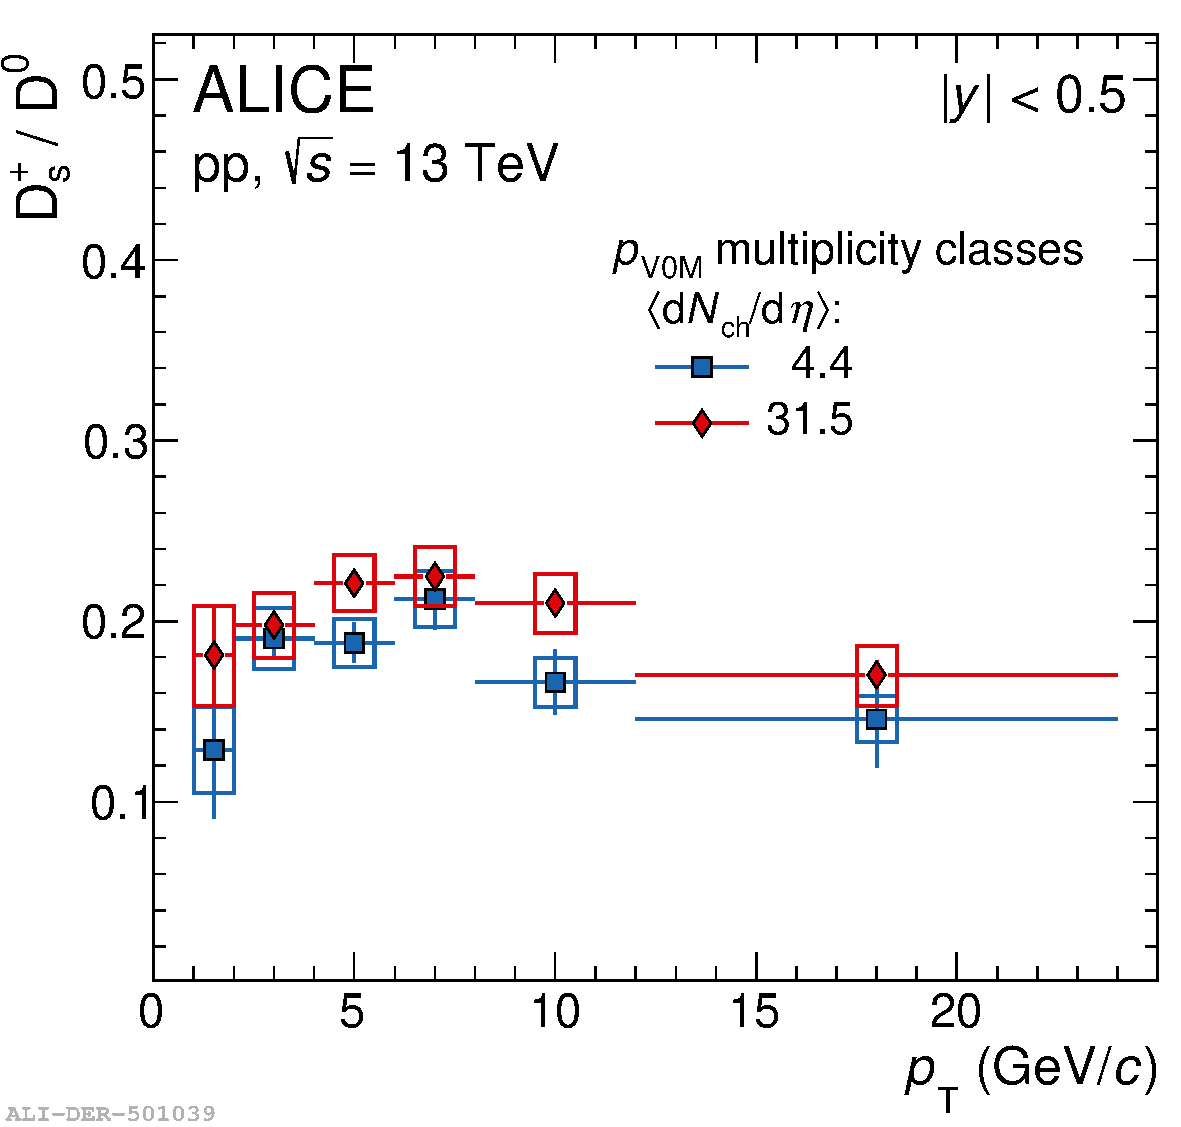
\includegraphics[width=0.7\textwidth]{Figures/Chapter 9/DsD0Ratios_LowHighMult_V0M_Derived.pdf}
    \caption{Strange over non-strange \ds/\dz production-yield ratio as a function of \pt for two different multiplicity classes measured at midrapidity ($\lvert y\rvert<0.5$) in proton-proton collisions at $\sqs=13$~\tev by the ALICE Collaboration~\cite{ALICE:2021npz}. Figure taken from the ALICE figure repository~\cite{ALICE_figures}.}
    \label{fig:ALICE_DsD0VsMultiplicity}
\end{figure}

Previous measurements of the multiplicity-dependence of the strange over non-strange \ds/\dz production-yield ratio in different multiplicity intervals performed at midrapidity ($\lvert y\rvert<0.5$) by the ALICE Collaboration~\cite{ALICE:2021npz} did not provide a clear indication of the strangeness enhancement in proton-proton collisions at $\sqs=13$~\tev. The results are illustrated in Fig.~\ref{fig:ALICE_DsD0VsMultiplicity}, where the measured \ds/\dz production-yield ratio is shown as a function of \pt for two different multiplicity classes. The results show a slight increase of the \ds/\dz production-yield ratio with the charged-particle multiplicity, although the two \pt-differential measurements are compatible within their uncertainties. The methodologies and results presented in this Thesis provide a solid foundation for future studies of the strangeness enhancement in the heavy-flavour sector. The strategy of using the \dpl meson as a reference for the non-strange production, as well as the reconstruction of both \ds and \dpl mesons in the same hadronic decay channel allows for a significant reduction of the systematic uncertainties of the measurement. The measurement of the multiplicity dependence of the \ds/\dpl production-yield ratio along with the larger data samples that will be available from the LHC Run~3 data-taking period may provide more precise results than those achieved through the usage of the \dz meson as a reference for non-strange D meson production, and, thereby, provide a more sensitive probe to the phenomenon of strangeness enhancement in proton-proton collisions. Additionally, the much larger data sample collected during the LHC Run~3 data-taking period will allow for the extension of the measurement to lower \pt values and perform the measurement in finer intervals of \pt and multiplicity.

%\begin{figure}[tb]
%    \centering
%    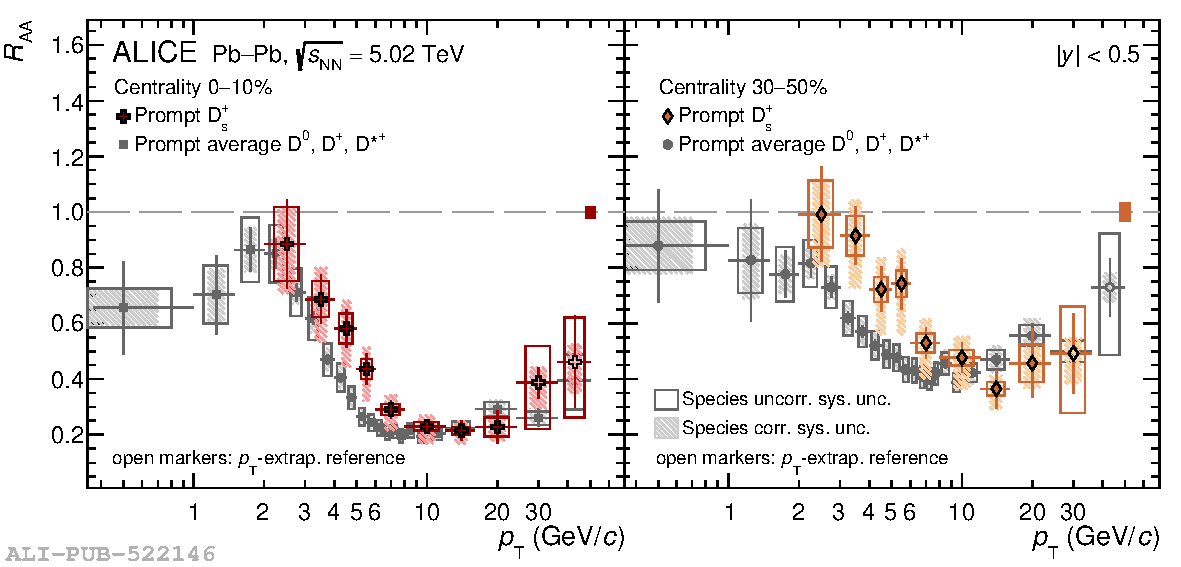
\includegraphics[width=\textwidth]{Figures/Chapter 9/PromptDs_vs_PromptD_Raa_2pads_1.pdf}
%    \caption{\raa of prompt \ds meson and average \raa of prompt \dz, \dpl, and $\mathrm{D^{*+}}$ mesons %as a function of \pt for the 0--10\% (left panel) and 30--50\% (right panel) centrality classes %measured at midrapidity ($\lvert y\rvert<0.5$) in Pb--Pb collisions at \mbox{$\snn=5.02$~\tev} by the %ALICE Collaboration~\cite{ALICE:2021npz}.}
%    \label{fig:RAA_Ds}
%\end{figure}

\begin{sloppypar}
The multiplicity phase space can be further explored by measuring the strange over non-strange D meson production-yield ratio in Pb--Pb collisions, where much higher charged-particle multiplicities are reached. Previous measurements performed by the ALICE experiment at a centre-of-mass energy per nucleon pair of \mbox{$\snn=5.02$~\tev~\cite{ALICE:2021kfc}} did not allow to draw firm conclusions on the possible enhancement of strange-hadron production in the charm sector. %Figure~\ref{fig:RAA_Ds} shows the nuclear modification factor \raa of prompt \ds mesons, compared to the average \raa of prompt \dz, \dpl, and $\mathrm{D^{*+}}$ mesons, as a function of \pt. Results from the 0--10\% and 30--50\% centrality classes are shown in the left and right panels, respectively. The measured \raa of prompt \ds mesons in Pb--Pb collisions is compatible within uncertainties with that of other non-strange D mesons for $\pt\gtrsim10$\gevc, where the hadronisation process is expected to occur mainly via fragmentation. At lower \pt, where the coalescence mechanism is expected to play a more relevant role, the measured \raa of prompt \ds mesons is systematically higher than that of non-strange D mesons, although the results are compatible within one standard deviation for both central and semicentral collisions.
\end{sloppypar}


\begin{figure}[htb]
    \centering
    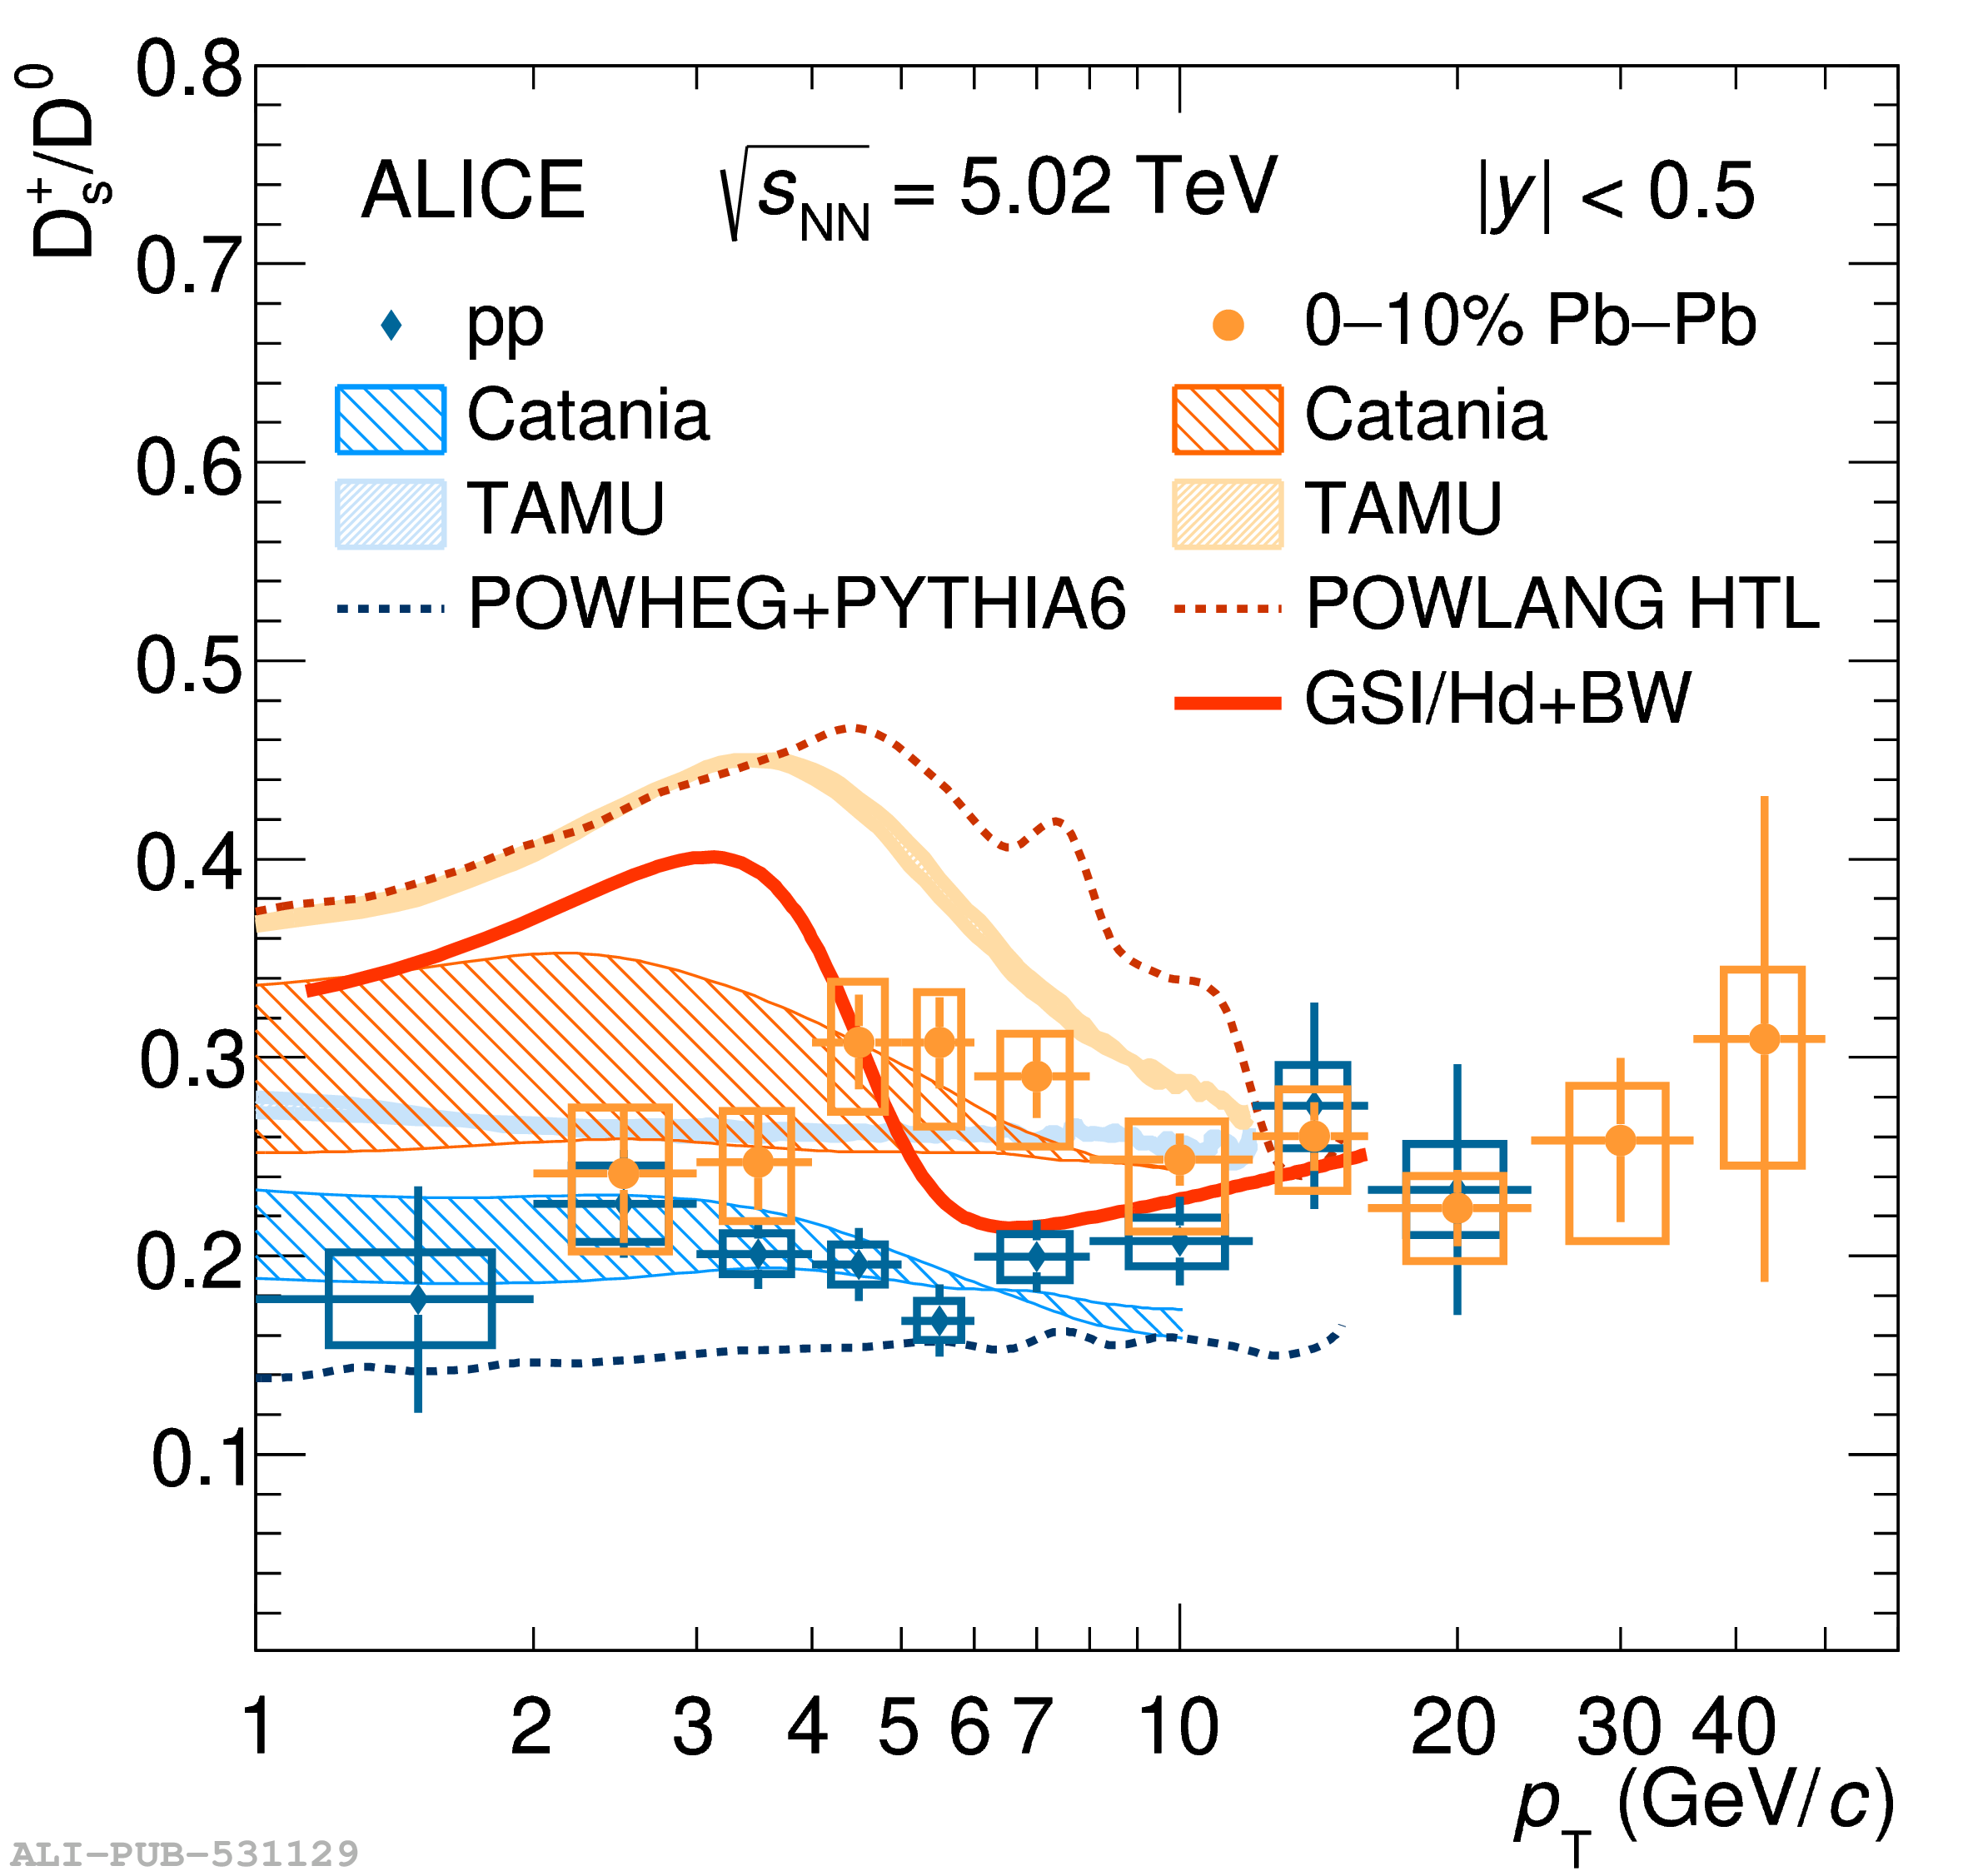
\includegraphics[width=0.7\textwidth]{Figures/Chapter 9/DsOverD0_pp_PbPb_5dot02TeV.png}
    \caption{\ds/\dz production-yield ratio as a function of \pt in pp collisions and in the 10\% most central \pbpb collisions at $\snn=5.02$~\tev compared to different model calculations. Figure taken from Ref.~\cite{ALICE:2022wpn}.}
    \label{fig:Double_ratio}
\end{figure}

The results from the measurement of the \ds/\dz production-yield ratios in central (0--10\%) Pb--Pb collisions compared to pp collisions are shown in Fig.~\ref{fig:Double_ratio}. While the measured ratio is consistent within the uncertainties between the two collision systems for $\pt<4$~\gevc and $\pt>8$~\gevc, the average values of the measured \ds/\dz production-yield ratio in the $2 < \pt < 8$~\gevc interval in Pb--Pb collisions are larger than those in pp collisions by about $2.3\sigma$ of the combined statistical and systematic uncertainties.

The results are also compared to different theoretical predictions. The Catania model~\cite{Plumari:2017ntm,Scardina:2017ipo}, already introduced in Chapter~\ref{ch:openHF} for pp collisions, assumes that a colour-deconfined state of matter is formed in both pp and Pb--Pb collisions and implements the heavy-quark transport via the Boltzmann equation. The hadronisation can occur via instantaneous coalescence, in addition to the fragmentation. In the TAMU~\cite{He:2019vgs} model, a combined recombination and fragmentation approach is implemented. The former is realized in Pb--Pb via the Resonance Recombination Model (RRM)~\cite{Ravagli:2007xx} where the recombination probability for the two-body case is controlled by resonance amplitudes and is expressed as a relativistic Breit-Wigner cross-section. In pp collisions, the abundances of the different charm-hadron species are instead determined with a statistical hadronisation approach~\cite{He:2019tik}. The charm-quark transport in a hydrodynamically expanding medium
is described by the Langevin equation. POWHEG~\cite{Frixione:2007nw} NLO pQCD calculations for the charm-quark productuction, matched with \textsc{Pythia}~6 to generate the parton shower are reported for pp collisions. Predictions from the GSI-Heidelberg Statistical Hadronisation Model~\cite{Andronic:2021erx} and POWLANG~\cite{Beraudo:2014boa} with transport coefficients calculated with weak-coupling calculations~\cite{Braaten:1989mz} (Hard-Thermal-Loop, HTL) are shown for Pb--Pb collisions. In the former, the \pt spectra of charm hadrons are modelled with a core-corona approach. In the low-\pt region, the charm production is dominated by the core contribution, described with a Blast Wave function, which is used to describe the velocity profile of the collectively expanding system, as introduced in Chapter~\ref{ch:QGP}. The corona contribution is parametrised from measurements in pp collisions and is relevant at high \pt. The \pt-spectra modification due to resonance decays is computed using the FastReso package~\cite{Mazeliauskas:2018irt}. In the latter, a Langevin-based transport of heavy quarks in the QGP is followed by in-medium hadronisation. At the hadronisation stage charm quarks are recombined with light thermal quark or di-quark states from the medium into colour-singlet clusters.

The Catania model reproduces within the uncertainties the measured \ds/\dz production-yield ratios both in pp and Pb--Pb collisions. The TAMU model overestimates the measured \ds/\dz ratio by a similar amount in the two colliding systems. A similar magnitude and \pt shape is predicted by the POWLANG model, while POWHEG calculations with \textsc{Pythia}~6 slightly underestimate the \ds/\dz production-yield ratio in pp collisions. The GSI-Heidelberg SHMc model provides a similar \pt shape for the \ds/\dz production-yield ratio as that provided by the TAMU and POWLANG models. The results do not allow for drawing firm conclusions on the phenomenon of strangeness enhancement in Pb--Pb collisions given the large uncertainties. However, they provide indications about the role of the charm-quark hadronisation via coalescence in the QGP.

The results discussed above do not allow for drawing firm conclusions on the phenomenon of strangeness enhancement in Pb--Pb collisions given the large uncertainties. The increase in the \ds/\dz porduction-yield ratio in the $2<\pt<8$~\gevc interval is compatible with the expectations from the modification of the charm-quark hadronisation in the presence of a deconfined medium and the phenomenon of strangeness enhancement. However, as also discussed in Chapter~\ref{ch:PbPb}, a measurement performed in the $\pt>2$~\gevc does not allow the disentanglenent of an enhancement in the \ds meson production from a difference in the momentum spectra in the two collision systems. Furthermore, the collective radial expansion of the medium may play a role in the increase of the \ds/\dz production-yield ratio in Pb--Pb collisions because of the different masses of the \ds and \dz mesons. Additionally, the studied centrality classes do not provide a complete picture of a possible trend in the production of strange hadrons as a function of the centrality of the collision (which, in turn, provides information on the partonic densities reached in the formed medium). A more comprehensive study would require to also explore both the intermediate centrality (10--30\%) and the most peripheral collisions (50--100\%), which could not be studied with the LHC Run~2 samples because of the limited number of recorded events.

The measurement of the double ratio of \ds/\dpl production-yield ratios in Pb--Pb and pp collisions will provide a clearer insight into the charm-quark hadronisation in a strangeness rich medium. This measurement would doubly benefit from the reduction of the systematic uncertainties from the reconstruction of both D meson species in the same decay channel, as the improvement would affect both the numerator (results in Pb--Pb collisions) and the denominator (results in pp collisions) of the double ratio. Additionally, the statistical uncertainties of the measurement will be significantly reduced thanks to the improved spatial resolution of the upgraded Inner Tracking System (ITS~2) and the larger data samples collected during the LHC Run~3. This will allow the extension of the measurement to lower \pt values, where the effects of the hadronisation via recombination are expected to be more pronounced, and to explore a wide multiplicity interval from pp collisions up to the most central Pb--Pb collisions. With these perspectives, the ALICE Collaboration will provide a state-of-the-art measurement of the strangeness enhancement in the heavy-flavour sector, with a comprehensive study of the hadronisation mechanisms of charm quarks in high-energy nuclear collisions.



